After the world wide web explosion at the ending of 1990's, Google has
emerged as one of the most significant web searching companies.
The novelty of Google was PageRank \cite{ilprints361}, an
algorithm counting the number of outgoing links of a webpage to determine its
importance. In order to apply the PageRank algorithm and form the
Google search results, first the webpage has to be scraped and
indexed. As of 2004 the raw size of the documents that had been
collected was more than 20 terabytes
\cite{Dean:2004:MSD:1251254.1251264}. Although the engineers at Google
have distributed and parallelized the algorithm, there were more tasks
that other teams have parallelized in a different way making it
difficult to maintain such a diverse codebase. That led them in 2004
to publish a paper about MapReduce, a generic framework to write distributed
applications that hide all the complexity of fault-tolerance, locality
awareness, load balancing etc.

MapReduce programming model borrows two very common functions from
functional programming, \emph{Map} and \emph{Reduce}. The \emph{Map}
function takes as input key/value pairs and produces as output a set
of key/value pairs as well. The \emph{Map} function is written by the
user and varies depending on the use case.

The \emph{Reduce} function, takes as input the
intermediate key/value pairs produced by \emph{Map} and merge them
together producing a smaller set of values. The \emph{Reduce} function
and the way it will merge the intermediate pairs is also provided by
the user.

A trivial example of the MapReduce programming model is that of
counting the occurrences of words in a text. The \emph{Map} function
takes as input a list of all the words in the text and emits tuples
in the form \texttt{(word,1)}, where \texttt{word} is every word
parsed. The result of the \emph{Map} function is passed to the
\emph{Reduce} function which adds the value of the tuples with the
same key, in that case is the word. The final result will be a list of
tuples with unique keys, where the key is all the words parsed from the text and the
value would be the occurrences of the word in the text.

Google provided a framework which took advantage of the locality
awareness of the already existing GFS and the MapReduce programming
paradigm. The execution overview of MapReduce is depicted in Figure
\ref{fig:mapreduce_execution_overview}. We can identify two entities
in MapReduce architecture, the \emph{Master} and the \emph{Workers}.

\begin{figure}
\centering
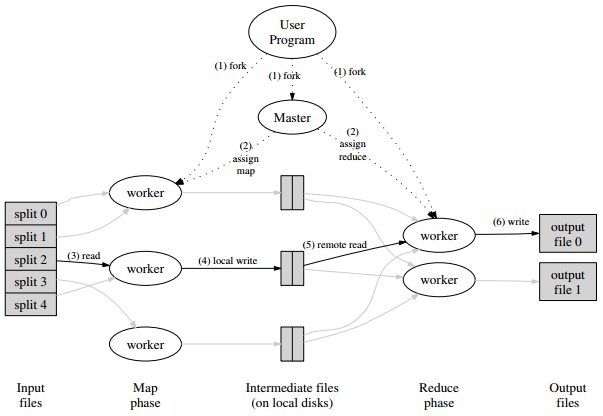
\includegraphics[scale=0.8]{resources/images/Background/mapreduce_exec_overview.png}
\label{fig:mapreduce_execution_overview}
\caption{MapReduce execution overview \cite{Dean:2004:MSD:1251254.1251264}}
\end{figure}

The \emph{Master} has the role of the coordinator that pushes the jobs
to the worker machines. It keeps track of the status of jobs in the
workers, informs other workers for the intermediate files produced
during the Map phase and pings the workers to verify their liveness.

The \emph{Workers} reside at the same physical hardware as the GFS
nodes to take advantage of the data locality. They are divided into
\emph{mappers}, which execute the Map function and \emph{reducers},
which perform the reduce phase as instructed. Workers are
pre-configured with available map or reduce slots depending on their
CPU or RAM.

At the very beginning, a user submits a job to Master. Master forks
the submitted job and is responsible to schedule the forks on workers
that $(a)$ have available map/reduce slots and $(b)$ have the
requested datasets stored locally. Upon the scheduling is done, the
Map phase begins in the mappers. They read the datasets from the local
hard drive and perform the Map function. Master periodically pings the
mappers to get informed about the status of the job and the health of
the node itself. When a mapper node completes its task, it writes the
intermediate key/value pairs to the local file system and informs the
Master node. The Master node in turn, notifies the reducer nodes that
an intermediate result is available at a specific node, where the
latter reads it (the result) remotely and perform the reduce
function. Finally, when all the reducers have completed the Reduce
phase, the Master notifies the user program.

\subsubsection{MapReduce Fault Tolerance}
Primary concern of the engineers was the fact
that machines will eventually fail. MapReduce will run on a cluster of
thousands of machines so the probability of a failed one would be
higher. For that reason they equipped MapReduce with a heartbeating
mechanism in order to be able to handle such situations.
The Master periodically pings the workers. The workers should respond back
within a predefined timeout before they are declared dead. When a node
that performs the Map phase is declared dead, the job that was
running at that node is set to \emph{idle} and is rescheduled on
another node. Similarly, when a map job has finished, since the
intermediate result is written to the local hard drive, the job has to
be rescheduled in a different machine. When a reducer node has failed
and the job is still in \emph{running} state, then it is set back in
\emph{idle} state and assigned to another node. In case of a completed
Reduce phase, the result is stored in the global file system, GFS in
that case. So, even with a failed reducer machine, the result will
still be available and the job should not be rescheduled.

While a Worker failure does not greatly affect the MapReduce job, it
is not the same case with a Master failure. If a machine that is a
Master node fails, then the whole MapReduce job is canceled and the
client is informed so that it can retry later on. ``However, given
that there is only a single master, its failure is unlikely;''
\cite{Dean:2004:MSD:1251254.1251264}.

\subsubsection{Limitations}
\label{sssec:mapreduce_limitations}
MapReduce facilitated engineers to ``easily'' write parallel data
processing applications by hiding all the complexity of a distributed
system. It provided some sort of fault tolerance and it was generic
enough to fit in various domains.

MapReduce and Hadoop over the years has become the industry standard
for processing and storing big volumes of data. After some period of
heavy usage it became clear that, although the platform itself suited
the needs for distributed, reliable storage and cluster management,
there were some limitations that had to be addressed. The two key
shortcomings were regarding the tight coupling of a programming model
with the resource management infrastructure and the centralized
handling of jobs \cite{Vavilapalli:2013:AHY:2523616.2523633, 6680946}.

A user who wantsto write an application for MapReduce framework,
all it has to do is to provide implementation for the two
first-order functions \emph{Map} and \emph{Reduce}. This static
map-reduce pipeline is very limiting though, as every job should have exactly one
Map function followed by an optional Reduce function. That workflow is
not suitable for large scale computations, such as machine learning
programs that require multiple iterations over a dataset. That means
that multiple individual MapReduce jobs have to be scheduled while the
frequent write of data in disk or in a distributed file system would
impose a considerable latency. A common pattern/misuse
\cite{Vavilapalli:2013:AHY:2523616.2523633} was to submit jobs with a
map phase only that spawned alternative frameworks or even web
servers. The scheduler had no semantics about the job except that they
were map jobs with a consequence in the cluster utilization, creating
deadlocks and a general instability to the system. The second drawback
of MapReduce and Hadoop 1.x was the centralized job handling and
monitoring of their flow. The Master or the \emph{JobTracker} should
monitor every single job, receiving liveness heartbeats, resource
requests etc. The is a heavy workload for a single machine that drove
to major scalability issues.

These two crucial limitations of MapReduce led to a total re-design of
Hadoop. Since Hadoop 2.0 there is a resource management module, YARN --
\emph{Yet Another Resource Negotiator} which will be analyzed in
section \ref{ssec:yarn} and MapReduce is just another application
running on a cluster of physical machines.